\section{Calibration Data}
\label{sec:calibration_date}

\subsection{Twilight Flats}

Because the flat field screen and illuminator is not expected to be operational while ComCam is on the telescope, we used dithered, tracked twilight flats to generate the combined flat calibration frames. The exposure time of the twilight flats were dynamically adjusted to hit a target count, generally in the range of 10-20k. The flats taken at a wide range of azimuth angles and rotator angles. See Fig.~\ref{fig:twilight_counts} for the counts per pixel per second as a function of sun elevation angle.

\begin{figure}
  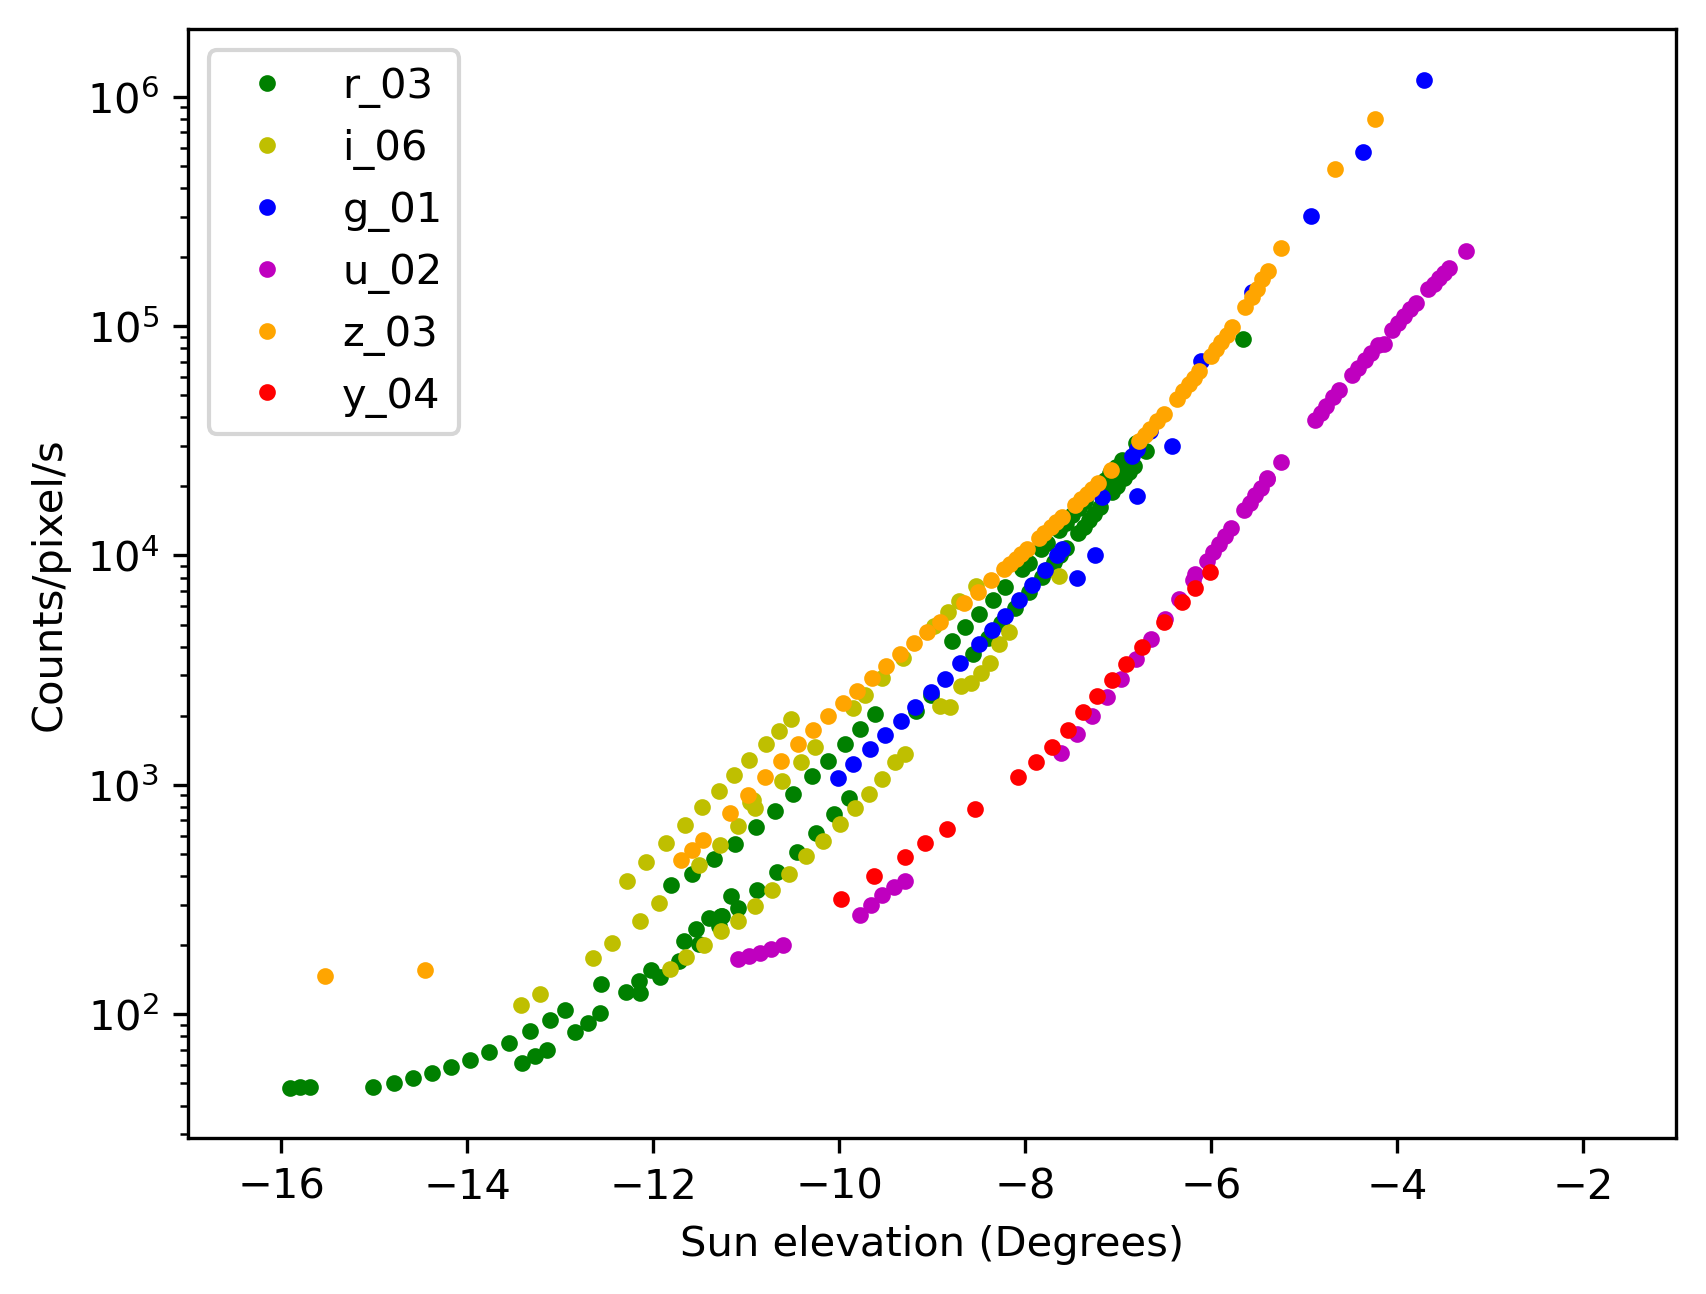
\includegraphics{calibration_data_figures/twilight_flat_counts.png}
  \caption{Twilight flat counts per pixel per second for each filter as a function of sun elevation angle.}
  \label{fig:twilight_counts}
\end{figure}
  